\section{Environment}
\label{sec:env}

The main focus of this work is deploy our \ac{LTR} framework in a subarctic environment and evaluate it's performance when subject to complex weather conditions.
In order to do so, we conducted our deployments within the \textit{Montmorency} boreal forest, located \SI{70}{km} North of \quebec~city, Canada.
Characteristics of boreal forests include dense closed-crown conifer vegetation~\citep{Russell1988} and long, cold winters leading to a high snow cover on the ground.
Dense vegetation is known to cause an issue for real-time mapping due to static antenna signal being blocked for \ac{RTK} \ac{GNSS}~\citep{Babin2019}.
Snow cover, illumination variation and the uniformity of the environment are also known to be challenging for vision-based approaches~\citep{Paton2017}.
Three different one-way paths were defined, all link 2 \acp{POI}.
The A  and B paths link the Garage and \laverdiere~\acp{POI} through cross-country ski trails, measuring \SI{1.5}{km} and \SI{1.5}{km} respectively.
In order to maximize \ac{UGV} and prevent immobilization, the A and B paths was previously driven on by a snowmobile operator.
The C path connects the Garage and Gazebo \acp{POI} mostly in a larger road network, measuring \SI{0.6}{km}.
The path network is illustrated in~\autoref{fig:forest}.

\begin{figure}[htpb]
	\begin{center}
		\begin{subfigure}[b]{0.45\textwidth}
			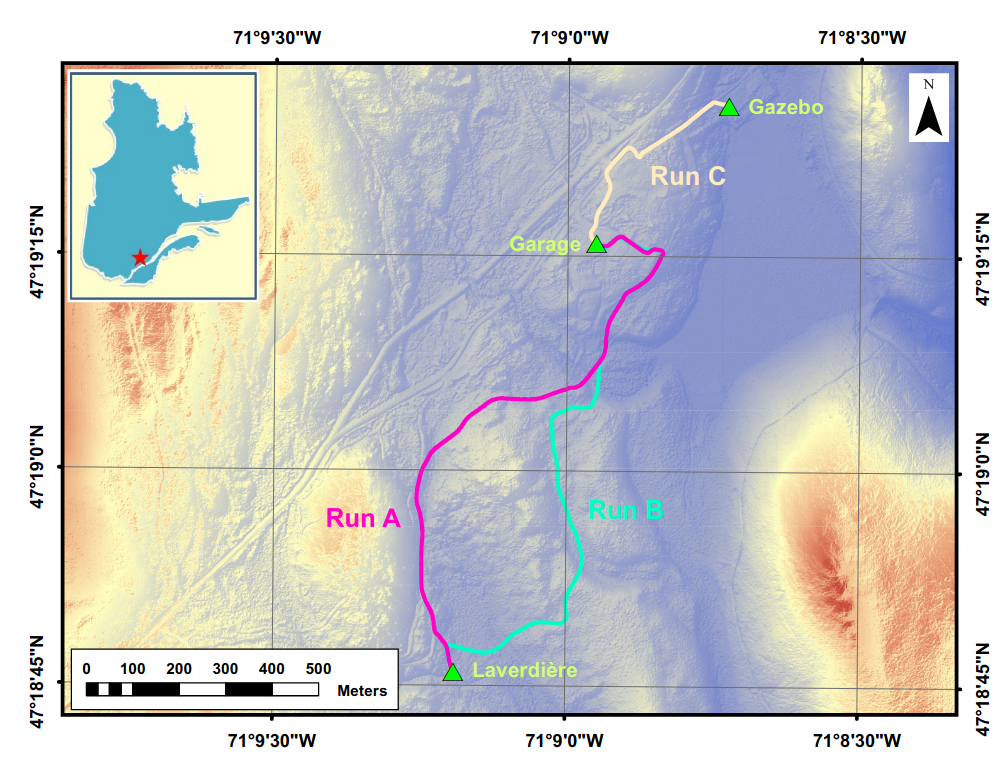
\includegraphics[width=\linewidth]{figs/fm_mnt.png}
			%\caption{A view from above the \textit{Montmorency} forest, which covers \SI{400}{km^2}.}
			\label{fig:view_above}
		\end{subfigure}%
		~~
		\begin{subfigure}[b]{0.45\textwidth}
			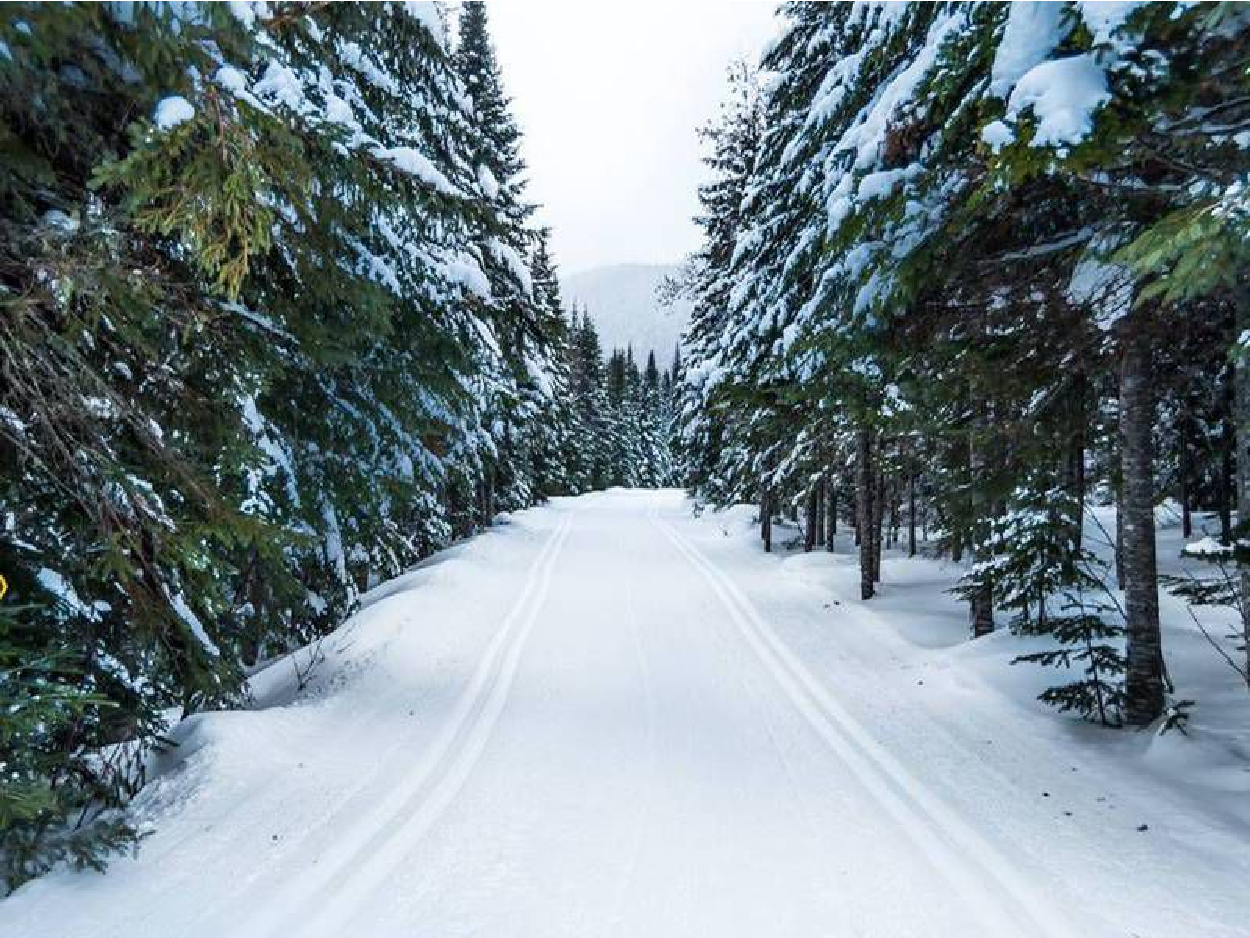
\includegraphics[width=\linewidth]{figs/foret-montmorency-path.pdf}
			%\caption{An example of a snowy path, in which our system performed \ac{LTR}.}
			\label{fig:view_path}
		\end{subfigure}%
		%% Maybe change with a camera image?
		\caption{A digital terrain model of the area where our \ac{LTR} system was deployed.
		We see the three different paths, both the A (\SI{1.5}{km}) and B path ({1.5}{km}) going from the garage \ac{POI} to the \laverdiere~\ac{POI}, while the C path (\SI{0.6}{km}) goes to the Gazebo \ac{POI}.
		The image on the right is an example of the A and B paths, which mostly consists of cross-country sky trails.
		Image credit : \foretmo.} 
		\label{fig:forest}
	\end{center}
\end{figure}

During the deployment, which lasted throughout five days, 

\begin{figure} [htpb]
	\centering
	\includegraphics[height=2.0in]{example-image}
	\caption{Johann's various runs and meteo figure}
	\label{fig:meteo_runs}
\end{figure}

\lightlipsum[1]